\documentclass{article}
\usepackage{geometry}
\geometry{margin=1in}
\usepackage{multirow}


%Figures
\usepackage{subcaption}
\usepackage{graphicx}
\usepackage{array}
\graphicspath{ {./images/} }

%Tables
\usepackage[table,xcdraw]{xcolor}
\usepackage{stfloats}
\usepackage{setspace}

\title{MAE 159 Midterm Aircraft Sizing Report}
\author{Thomas Slagle}
\date{May 7th, 2021}

\parskip=10pt

\begin{document}
    \maketitle

    \section{Introduction}
    \label{sec:intro}
    \begin{flushleft}
        This report consists of a study on the cost and performance optimization
        for two subsoinc commercial transport aircraft, one non-stop aircraft
        and one one-stop aircraft. Herein, the reader will find a summary of the
        methods used and the data generated from an itterative python script
        which uses standard, well-defined aircraft deisgn methods to exactly
        meet the design specifications. Various parameters, including the aspect
        ratio, the airfoil type, the wing sweep angle, and the seating
        configuration, were systematically varied to determine the optimum
        design parameters for each aircraft. In the conclusion of the report,
        the optimum aircraft design parameters will be given as well as a
        summary of why the design was chosen, and which of the two
        aircraft may suit the customer's needs the best.
    \end{flushleft}

    \section{Design Specifications}
    \label{sec:specs}
    \begin{flushleft}
        As mentioned prior, two aircraft with distinct given design
        requirements, were considered in this design study. Both aircraft are
        requried to carry 225 passangers and complete a 7400 nautical mile
        journey. The first larger aircraft must compelte the journey without any
        stops. The second smaller aircraft must complete the journey with
        one-stop, giving the airplane a required range of 3700 nautical miles.
        The complete set of given design specifications are listed in tables 1
        and 2 below. For both aircraft, takeoff conditions were assumed to be at
        sea level on a hot day with an air temperature of $84^{\circ}F$.
    \end{flushleft}

    \begin{table}[ht]
    \begin{tabular}{|c|c|}
    \hline
    \rowcolor[HTML]{FFC702}
    \multicolumn{2}{|c|}{\cellcolor[HTML]{FFC702}\textbf{Non-stop Aircraft}} \\ \hline
    \textbf{Design Specification:}        & \textbf{Parameter Value:}        \\ \hline
    Number of Passangers                  & 225                              \\ \hline
    \rowcolor[HTML]{C0C0C0}
    Weight of Cargo                       & 6,000 lbs                        \\ \hline
    Still Air Range                       & 7,400 nmi                        \\ \hline
    \rowcolor[HTML]{C0C0C0}
    Takeoff Field Length                  & 10,500 ft                        \\ \hline
    Landing Approach Speed                & 140 kts                          \\ \hline
    \rowcolor[HTML]{C0C0C0}
    Fuel Destination Payload              & 35\%                             \\ \hline
    Cruise Mach Number                    & 0.85                             \\ \hline
    \rowcolor[HTML]{C0C0C0}
    Initial Cruise Altitude               & 35,000 ft                        \\ \hline
    \end{tabular}
    \quad
    \begin{tabular}{|c|c|}
        \hline
        \rowcolor[HTML]{DAE8FC}
        \multicolumn{2}{|c|}{\cellcolor[HTML]{DAE8FC}\textbf{One-stop Aircraft}} \\ \hline
        \textbf{Design Specification:}        & \textbf{Parameter Value:}        \\ \hline
        Number of Passangers                  & 225                              \\ \hline
        \rowcolor[HTML]{C0C0C0}
        Weight of Cargo                       & 3,000 lbs                        \\ \hline
        Still Air Range                       & 3,700 nmi                        \\ \hline
        \rowcolor[HTML]{C0C0C0}
        Takeoff Field Length                  & 6,000 ft                         \\ \hline
        Landing Approach Speed                & 130 kts                          \\ \hline
        \rowcolor[HTML]{C0C0C0}
        Fuel Destination Payload              & 0\%                              \\ \hline
        Cruise Mach Number                    & 0.80                             \\ \hline
        \rowcolor[HTML]{C0C0C0}
        Initial Cruise Altitude               & 35,000 ft                        \\ \hline
    \end{tabular}
    \end{table}

    \section{Design Analysis}
    \label{sec:design}
    \begin{flushleft}
        The object of this section is to perform an analysis for both aircraft
        and determine the optimized specifications for the design parameters. An
        itterative python script was developed with allowable user input for
        user-selectable design parameters to make calculations of direct
        operating cost (DOC), weight, drag, and other airfact performance
        charactersitics easy, fast, and repeatable.
    \end{flushleft}

    \subsection{Direct Operating Cost versus Aspect Ratio and Wing Sweep Angle}
    \label{sec:AR}
        \begin{flushleft}
            The aspect ratio describes the ratio of the airfact's wingspan to
            its mean aerodynamic chord length. A small aspect ratio describes a
            short and wide wing whereas a larger aspect ratio describes a long
            and narrow wing planform. The wing aspect ratio is an important
            factor in determing the available lift of the aircraft, the weight
            of the aircraft, and the induced drag during flight. For a typical
            jet transport aircraft, Schaufele gives an aspect ratio range of 7.0
            to 9.5, as such, this formed the basis for design selection. Aspect
            ratios in steps of 0.1 were considered from 6.0 to 12.0 during this
            study. The method for comparison will be the resulting DOC per
            passanger, per mile. Figure \ref{fig:doctmAR} shows the aspect ratio
            versus the DOC with curves of fixed sweep angle for both the short
            range and long range aircraft. The fixed sweep angle curves are
            shown in steps of 1 degree. Each plot in \ref{fig:doctmAR} shows a
            total of 1800 discrete aircraft designs. All aircraft deisgns in
            this analysis utilized two JT9D engines and had one aisle with six
            abreast for the seating configuration.

            \begin{figure*}[ht]
                \centering
                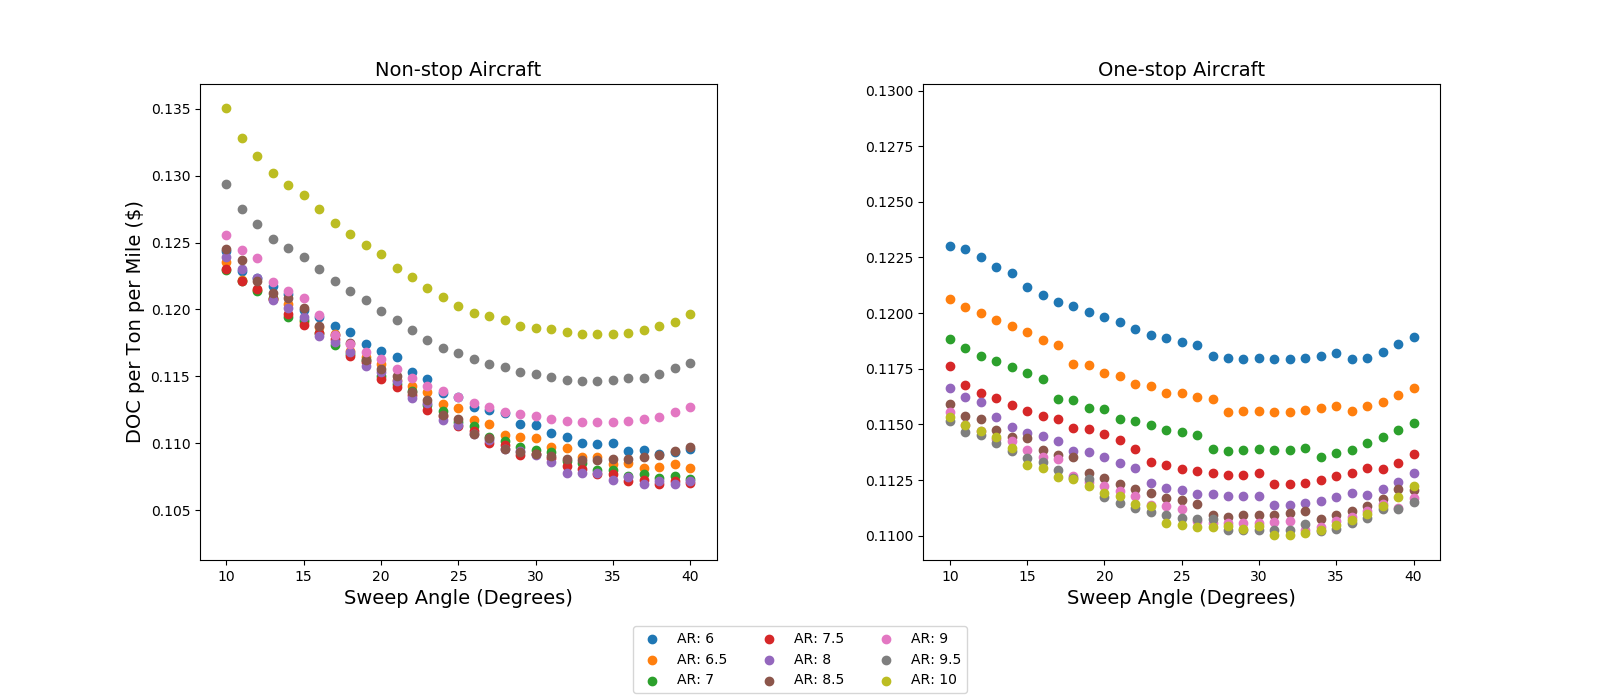
\includegraphics[scale=0.54]{DOCTM v Sweep Angle.PNG}
                \caption{Direct operating cost, per ton, per mile plotted against aspect ratio for the non-stop and one-stop aircraft at different wing sweep angles.}
                \label{fig:doctmAR}
            \end{figure*}

            From figure \ref{fig:doctmAR}, the optimized aspect ratio can be
            determined by finding the range at which the minimum value occurs.
            Due to the number of unique aircraft designs considered in this
            section of the study, a zoomed in version is presented in
            \ref{fig:doctmAR}. The nonstop aircraft plot is zoomed in on the 7.0
            to 8.2 aspect ratio range and the onestop aircraft plot is zoomed in
            on the 9.0 to 10.2 aspect ratio range.

            \begin{figure*}[ht]
                \centering
                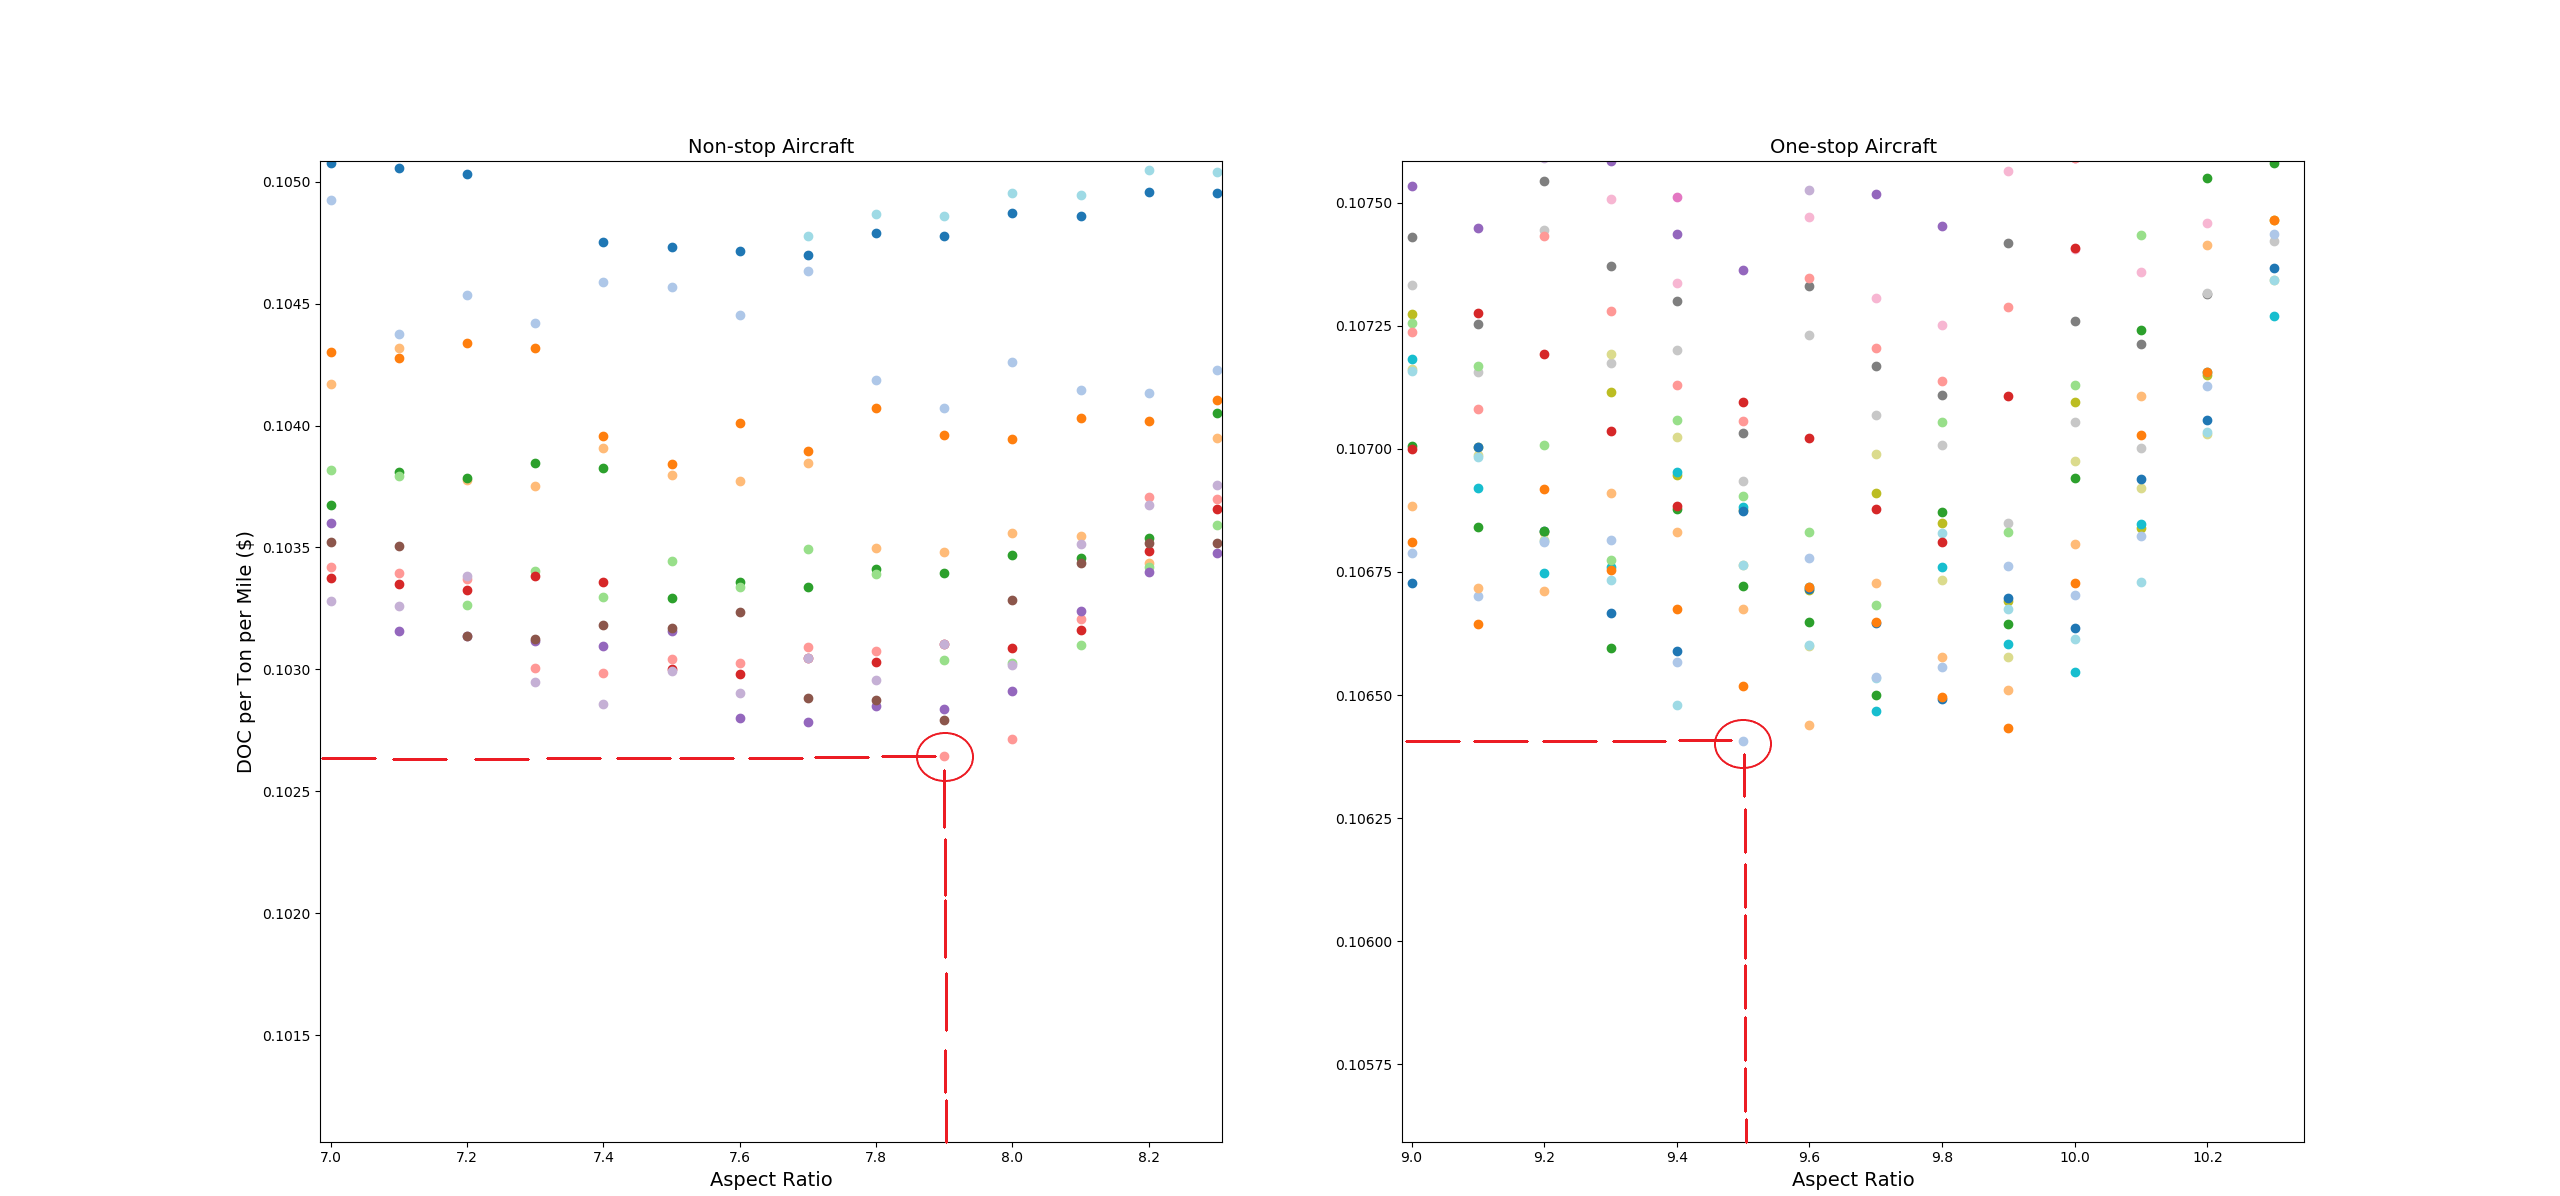
\includegraphics[scale=0.244]{DOCTM v Sweep Angle Zoom.PNG}
                \caption{Zoom of the direct operating cost, per ton, per mile plotted against aspect ratio for the non-stop and one-stop aircraft at different wing sweep angles.}
                \label{fig:doctmARzoom}
            \end{figure*}

            From this analysis, it is evident that for the non-stop aircraft,
            the optimized aspect ratio is 7.9 with a wing swep angle of 37
            degrees. For the one-stop aircraft, the optimized aspect ratio is
            9.5 with a wing sweep angle of 31 degrees. This corresponds to a
            direct operating cost, per ton, per mile of \$0.1064 and \$0.1026
            for the onestop and nonstop aircraft respectively. The rest of the
            sections within section \ref{sec:design} will be based off of the
            control values found herein this section.
        \end{flushleft}

    \subsection{Weight versus Aspect Ratio and Wing Sweep Angle}
    \label{sec:weight}
        \begin{flushleft}
            Now that the most effiecnt plane in terms of cost to operate has
            been found, it is of interest to look at the weight of the aircraft
            and also the amount of fuel that is burned during flight. Figure
            \ref{fig:AR} plots the takeoff weight of the aircraft in pound versus the
            aspect ratio using fixed lines of sweep angle. The plots in this
            figure show a much more dramatic divergence from the optimum value
            than the direct operating cost plots. The minimum weight values
            occur near the range of aspect ratios for the lowest direct
            operating cost.

            \begin{figure*}[ht]
                \centering
                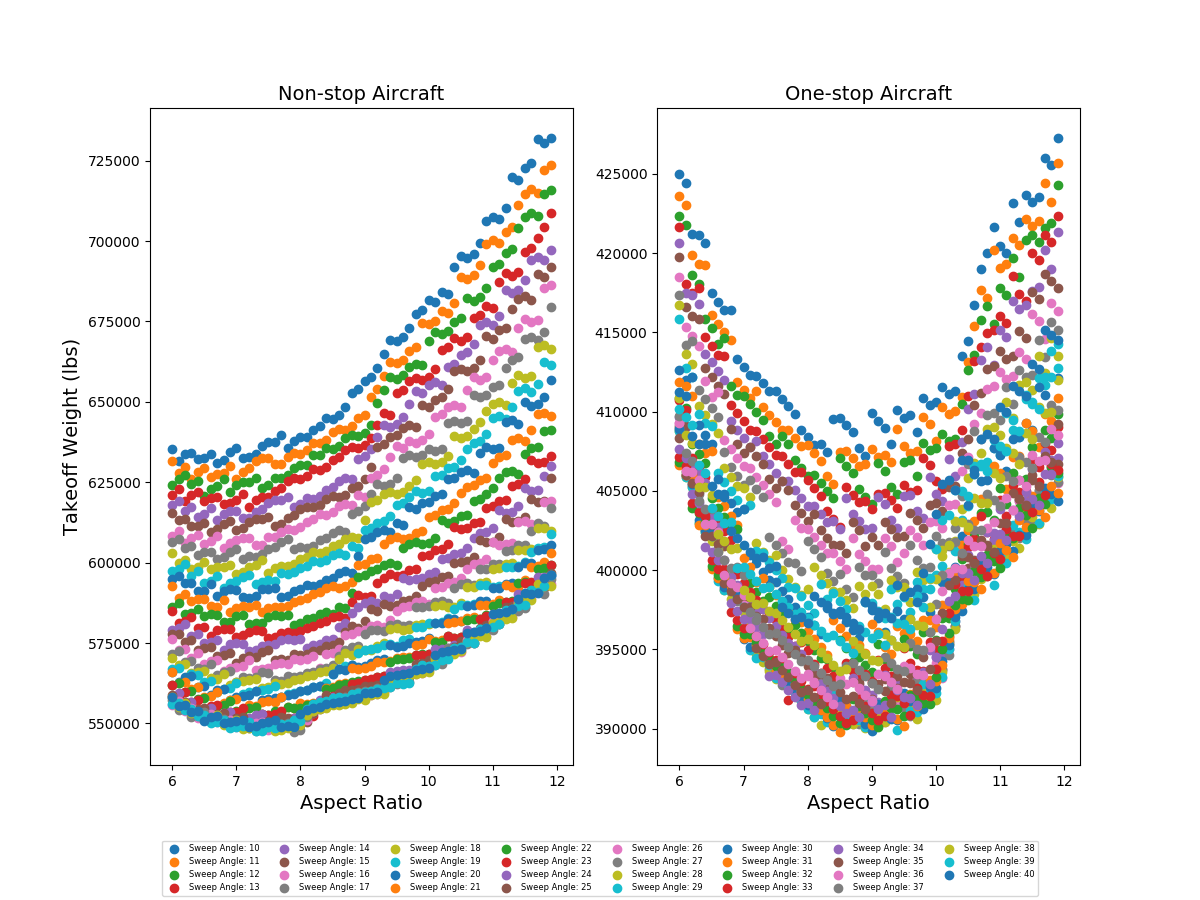
\includegraphics[scale=0.54]{Weight v Sweep Angle.PNG}
                \caption{Direct operating cost, per ton, per mile plotted against sweep angle for the non-stop and one-stop aircraft at the optimized aspect ratios.}
                \label{fig:AR}
            \end{figure*}

            A large fraction of the weight of the aircraft comes in the form of the weight of fuel required to make the distance.

        \end{flushleft}

    \subsection{Advanced Technology}
    \label{sec:adv_tech}
        \begin{flushleft}
            Modern technology and manufacturing advancements has allowed for the
            use of more exotic airfoil shapes and airframe materials that
            previous heritage aircraft could not take advantage of. Regarding
            airfoil selection, the advent of supercritical airfoils has been
            cited to improve aircraft fuel efficiency and thus lower the direct
            operating cost of the aircraft. The Boeing 757 and 767, developed
            during the 1980s were some of the first commerical aircraft to use
            this technology. However, these airfoils types are comprised of more
            complciated compund curves which presents added complexity in the
            manufacturing process, driving up initial cost of the aircraft
            however, the decrease in operational costs of the aircraft exceeds
            the initial procurement cost increase of the aircraft.

            The second advanced technology considering during the design process
            was the implementation of composites for the airframe materials.
            Airframes have typically been composed of various aluminum alloys
            which presents a strong yet lightweight option. However, recent
            advancements in materials engineering has allowed for reliable
            implementation of composite layups, which are lighter and stronger
            than the aluminum alternative. However, the process to form
            strucutres from composites is complicated and if not performed
            properly, the composite sturcutres may exhibit delamination.
            Performing the process correctly is expensive and time consuming,
            thus driving up the initial procrument costs of the aircraft using
            this technology. However, the savings in direct operating costs may
            offset this initial procrument price.

            Figure \ref{fig:doc} plots the direct operating cost of the aircraft
            using the optimized aspect ratio and wing sweep angle found in
            section \ref{sec:AR}, with the implementation of different
            technology improvements. Figure \ref{fig:weight} plots the takeoff weight of
            the aircraft with different technologies.

            \begin{figure*}[ht]
                \centering
                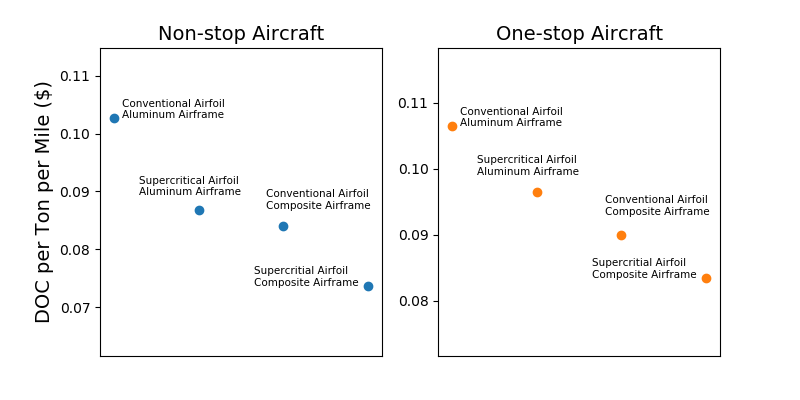
\includegraphics[scale=0.7]{tech.PNG}
                \caption{Direct operating cost, per ton, per mile for the optimal aircraft configration using different technologies.}
                \label{fig:doc}
            \end{figure*}

            \begin{figure*}[ht]
                \centering
                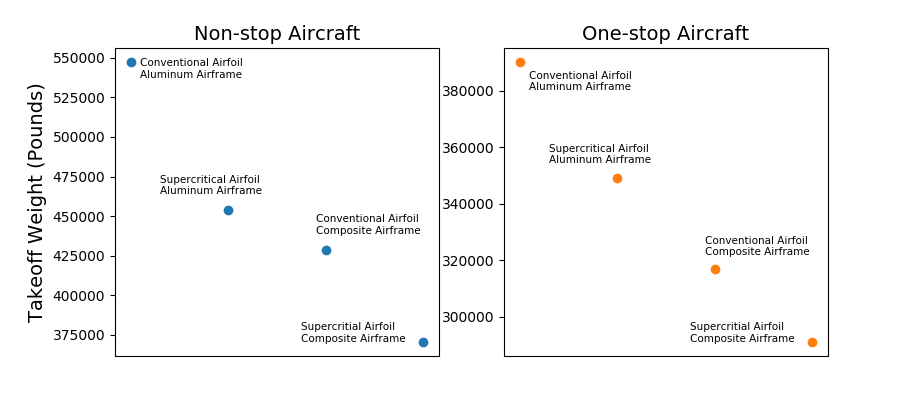
\includegraphics[scale=0.7]{tech_weight.PNG}
                \caption{Takeoff Weight for the optimal aircraft configration using different technologies.}
                \label{fig:weight}
            \end{figure*}

            It is clear that both technologies, supercritical airfoils and
            composite strucutres, reduce the direct operating cost. Using them
            together drives down the operating cost and weight of the aircraft
            dramaticaly.

        \end{flushleft}

    \subsection{Aircraft Seat Configuration}
    \label{sec:seat configuration}
        \begin{flushleft}
            The aircraft seat configuration can also be varied in the number of
            aisles that run the length of the fuselage, and the number of seats
            abreast. In this case, the main metric of comparison will be the
            direct operating cost. For this study, the optimized aspect ratio
            and both supercritical airfoil technology and composite technology
            has been applied to the aircraft design. In the previous sections, the
            standard configuration of one aisle and six passangers abreast
            was considered. These results are plotted in figure \ref{fig:seats}.

            \begin{figure*}[ht]
                \centering
                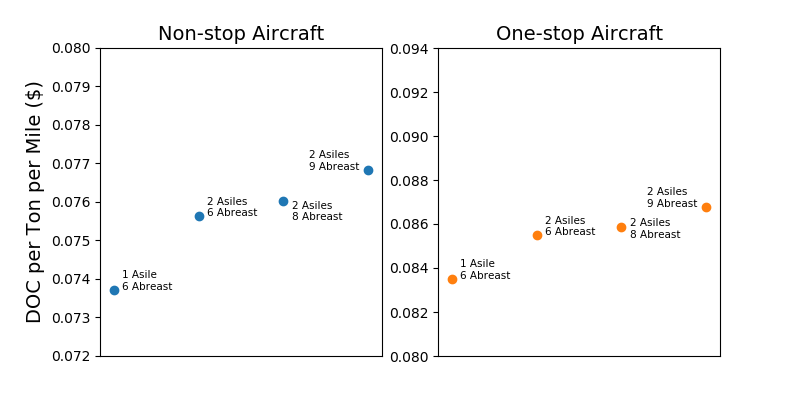
\includegraphics[scale=0.7]{seating.PNG}
                \caption{Direct operating cost, per ton, per mile for the optimal aircraft configration using different seating configurations.}
                \label{fig:seats}
            \end{figure*}

            From this study, it is evident that when holding the number of
            aisles constant, increasing the number of passangers abreast leads
            to a higher direct operating cost. Additionaly, it is clear that the
            one asile, six abreast configuration had a lower direct operaing
            cost for both aircraft than any of the two aisle configurations.
            However, the two aisle configuration has been found to have an
            advantage over a one aisle configuration in the fact that passangers
            are able to load and unload from the aircraft more quickly,
            signifigantly reducing the down time requried when at the airports.
            For aircraft that may be making shorter flights, such as the
            one-stop aircraft in this study, it may be more beneficial to use
            the two-aisle configuration despite the higher direct operating cost
            found in this study. The increased loading and unloading efficnecy
            was not taken into account in the direct operating cost estimation
            used in this study.

        \end{flushleft}


    \pagebreak
    \section{Summary and Conclusion}
    \label{sec:conclusion}
        \begin{flushleft}
            This section will summarize the results of the non-stop and one-stop
            aircraft design studies discussed in detail in the previous sections
            herein. Recommendations shall be made as to which aircraft may suit a
            given customer's needs the best.
        \end{flushleft}
    \subsection{Final Aircraft Design Specifications}
    \label{sec:optimized}
        \begin{flushleft}
            The table below lists the final optimized specifications of the non-stop and one-stop aircraft.

            \begin{table}[ht]
                \begin{tabular}{|c|c|}
                \hline
                \rowcolor[HTML]{FFC702}
                \multicolumn{2}{|c|}{\cellcolor[HTML]{FFC702}\textbf{Non-stop Aircraft}} \\ \hline
                \textbf{Design Specification:}        & \textbf{Parameter Value:}        \\ \hline
                Number of Passangers                  & 225                              \\ \hline
                \rowcolor[HTML]{C0C0C0}
                Weight of Cargo                       & 6,000 lbs                        \\ \hline
                Still Air Range                       & 7,400 nmi                        \\ \hline
                \rowcolor[HTML]{C0C0C0}
                Takeoff Field Length                  & 10,500 ft                        \\ \hline
                Landing Approach Speed                & 140 kts                          \\ \hline
                \rowcolor[HTML]{C0C0C0}
                Fuel Destination Payload              & 35\%                             \\ \hline
                Cruise Mach Number                    & 0.85                             \\ \hline
                \rowcolor[HTML]{C0C0C0}
                Initial Cruise Altitude               & 35,000 ft                        \\ \hline
                \end{tabular}
                \quad
                \begin{tabular}{|c|c|}
                    \hline
                    \rowcolor[HTML]{DAE8FC}
                    \multicolumn{2}{|c|}{\cellcolor[HTML]{DAE8FC}\textbf{One-stop Aircraft}} \\ \hline
                    \textbf{Design Specification:}        & \textbf{Parameter Value:}        \\ \hline
                    Number of Passangers                  & 225                              \\ \hline
                    \rowcolor[HTML]{C0C0C0}
                    Weight of Cargo                       & 3,000 lbs                        \\ \hline
                    Still Air Range                       & 3,700 nmi                        \\ \hline
                    \rowcolor[HTML]{C0C0C0}
                    Takeoff Field Length                  & 6,000 ft                         \\ \hline
                    Landing Approach Speed                & 130 kts                          \\ \hline
                    \rowcolor[HTML]{C0C0C0}
                    Fuel Destination Payload              & 0\%                              \\ \hline
                    Cruise Mach Number                    & 0.80                             \\ \hline
                    \rowcolor[HTML]{C0C0C0}
                    Initial Cruise Altitude               & 35,000 ft                        \\ \hline
                \end{tabular}
                \end{table}

        \end{flushleft}

    \subsection{Payload Range}
    \label{sec:PR}

    \subsection{Recommendations Customer Selection and Beyond}
    \label{sec:Recommendations}
        \begin{flushleft}

        \end{flushleft}


\end{document}
